%%%%%%%%%%%%%%%%%%%%%%%%%%%%%%%%%%%%%%%%%%%%%%%%%%%%%%%%%%%%%%%%%%%%%%%%%%%%
% AGUJournalTemplate.tex: this template file is for articles formatted with LaTeX
%
% This file includes commands and instructions
% given in the order necessary to produce a final output that will
% satisfy AGU requirements, including customized APA reference formatting.
%
% You may copy this file and give it your
% article name, and enter your text.
%
% guidelines and troubleshooting are here: 

%% user added for convenience, can be removed before submission:



%% To submit your paper:
\documentclass[draft]{agujournal2019}
\usepackage{url} %this package should fix any errors with URLs in refs.
\usepackage{lineno}
\usepackage[inline]{trackchanges} %for better track changes. finalnew option will compile document with changes incorporated.
\usepackage{soul}

% MY OWN ADDED PACKAGES TO RENDER UNITS
\usepackage{gensymb}
\usepackage{booktabs}

\linenumbers
%%%%%%%
% As of 2018 we recommend use of the TrackChanges package to mark revisions.
% The trackchanges package adds five new LaTeX commands:
%
%  \note[editor]{The note}
%  \annote[editor]{Text to annotate}{The note}
%  \add[editor]{Text to add}
%  \remove[editor]{Text to remove}
%  \change[editor]{Text to remove}{Text to add}
%
% complete documentation is here: http://trackchanges.sourceforge.net/
%%%%%%%

\draftfalse

%% Enter journal name below.
%% Choose from this list of Journals:
%
% JGR: Atmospheres
% JGR: Biogeosciences
% JGR: Earth Surface
% JGR: Oceans
% JGR: Planets
% JGR: Solid Earth
% JGR: Space Physics
% Global Biogeochemical Cycles
% Geophysical Research Letters
% Paleoceanography and Paleoclimatology
% Radio Science
% Reviews of Geophysics
% Tectonics
% Space Weather
% Water Resources Research
% Geochemistry, Geophysics, Geosystems
% Journal of Advances in Modeling Earth Systems (JAMES)
% Earth's Future
% Earth and Space Science
% Geohealth
%
% ie, \journalname{Water Resources Research}

\journalname{Enter journal name here}


\begin{document}

%%%%%%%%%%%%%%%%%%%%%%%%%%%%%%%%%%%%%%%%%%%%%%%
%  TITLE
%
% (A title should be specific, informative, and brief. Use
% abbreviations only if they are defined in the abstract. Titles that
% start with general keywords then specific terms are optimized in
% searches)
%
%%%%%%%%%%%%%%%%%%%%%%%%%%%%%%%%%%%%%%%%%%%%%%%

% Example: \title{This is a test title}

\title{Climate-driven Phytoplankton community variability in the Cariaco Basin, Venezuela}

%%%%%%%%%%%%%%%%%%%%%%%%%%%%%%%%%%%%%%%%%%%%%%%
%
%  AUTHORS AND AFFILIATIONS
%
%%%%%%%%%%%%%%%%%%%%%%%%%%%%%%%%%%%%%%%%%%%%%%%

% Authors are individuals who have significantly contributed to the
% research and preparation of the article. Group authors are allowed, if
% each author in the group is separately identified in an appendix.)

% List authors by first name or initial followed by last name and
% separated by commas. Use \affil{} to number affiliations, and
% \thanks{} for author notes.
% Additional author notes should be indicated with \thanks{} (for
% example, for current addresses).

% Example: \authors{A. B. Author\affil{1}\thanks{Current address, Antartica}, B. C. Author\affil{2,3}, and D. E.
% Author\affil{3,4}\thanks{Also funded by Monsanto.}}

\authors{B. Post\affil{1,2}, E. Acevedo-Trejos\affil{3}, S. Chakraborty\affil{1}, A.D. Barton\affil{4}, A. Merico\affil{1}}


% \affiliation{1}{First Affiliation}
% \affiliation{2}{Second Affiliation}
% \affiliation{3}{Third Affiliation}
% \affiliation{4}{Fourth Affiliation}

\affiliation{1}{Systems Ecology Group, Leibniz Centre for Tropical Marine Research (ZMT), Bremen, Germany}
\affiliation{2}{School of Science, Constructor University, Bremen, Germany}
\affiliation{3}{Earth Surface Process Modelling, GFZ German Research Centre for Geosciences, Potsdam, Germany}
\affiliation{4}{Scripps Institution of Oceanography and Department of Ecology, Behavior and Evolution, University of California San Diego, La Jolla, CA, United States}
%(repeat as many times as is necessary)


% Corresponding author mailing address and e-mail address:

% (include name and email addresses of the corresponding author.  More
% than one corresponding author is allowed in this LaTeX file and for
% publication; but only one corresponding author is allowed in our
% editorial system.)

% Example: \correspondingauthor{First and Last Name}{email@address.edu}

\correspondingauthor{Benjamin Post}{benjaminpost@aoop.de}



%%%%%%%%%%%%%%%%%%%%%%%%%%%%%%%%%%%%%%%%%%%%%%%
% KEY POINTS
%%%%%%%%%%%%%%%%%%%%%%%%%%%%%%%%%%%%%%%%%%%%%%%
%  List up to three key points (at least one is required)
%  Key Points summarize the main points and conclusions of the article
%  Each must be 140 characters or fewer with no special characters or punctuation and must be complete sentences

% Example:
% \begin{keypoints}
% \item	List up to three key points (at least one is required)
% \item	Key Points summarize the main points and conclusions of the article
% \item	Each must be 140 characters or fewer with no special characters or punctuation and must be complete sentences
% \end{keypoints}

\begin{keypoints}
\item The CARIACO time series showed a highly variable phytoplankton community over the course of sampling between 1995 and 2017. Clustering of community data from microscopy cell counts reveals two separate clusters, defined by high- and low-upwelling conditions that match the AMO index. 
\item Despite the differing physical regimes and the large changes between the functional groups, there are no significant differences in genus richness and Shannon diversity between the two clusters, although community evenness was higher in low upwelling conditions.
\item A gradient forest analysis of community data reveals that the strongest predictor of shifts within the community is the AMO index with a time lag of 2 months, pointing to a strong impact of large-scale climatic oscillations in the tropical coastal ecosystem. The next strongest predictor is the MEI v2 index (lag of 4 months), with in-situ temperature and nitrate concentration following behind. 
\end{keypoints}

%%%%%%%%%%%%%%%%%%%%%%%%%%%%%%%%%%%%%%%%%%%%%%%
%
%  ABSTRACT and PLAIN LANGUAGE SUMMARY
%
% A good Abstract will begin with a short description of the problem
% being addressed, briefly describe the new data or analyses, then
% briefly states the main conclusion(s) and how they are supported and
% uncertainties.

% The Plain Language Summary should be written for a broad audience,
% including journalists and the science-interested public, that will not have 
% a background in your field.
%
% A Plain Language Summary is required in GRL, JGR: Planets, JGR: Biogeosciences,
% JGR: Oceans, G-Cubed, Reviews of Geophysics, and JAMES.
% see http://sharingscience.agu.org/creating-plain-language-summary/)
%
%%%%%%%%%%%%%%%%%%%%%%%%%%%%%%%%%%%%%%%%%%%%%%%

%% \begin{abstract} starts the second page

\begin{abstract}
The structure of the phytoplankton community was identified using microscopy in the Cariaco basin, in Venezuela, between 1995 and 2017. Microscopy data are limited to larger cell sizes (> 20 µm), where the community showed a large change in the abundances of functional groups and shifts in diversity patterns. 
\end{abstract}

%1
%\section*{Plain Language Summary}
%Enter your Plain Language Summary here or delete this section.
%Here are instructions on writing a Plain Language Summary: 
%https://www.agu.org/Share-and-Advocate/Share/Community/Plain-language-summary


%%%%%%%%%%%%%%%%%%%%%%%%%%%%%%%%%%%%%%%%%%%%%%%
%
%  BODY TEXT
%
%%%%%%%%%%%%%%%%%%%%%%%%%%%%%%%%%%%%%%%%%%%%%%%

%%% Suggested section heads:
\section{Introduction}
%
% The main text should start with an introduction. Except for short
% manuscripts (such as comments and replies), the text should be divided
% into sections, each with its own heading.

% Headings should be sentence fragments and do not begin with a
% lowercase letter or number. Examples of good headings are:

    \begin{itemize}
    
        %% Overarching theme: Stability of Ecosystem faunctions, Drivers of community change
        
        \item "The Cariaco Basin, located ...." - general hydrography/depth, etc.
    
        \item "The CARIACO Time Series ...." - talk about the Time Series, what they did, why
    
        \item "The Cariaco Basin has undergone marked shifts..." Talk about ecosystem, what has changed, reference prev literature

        % below is from 2019 REVIEW
        Hydrographic observations (Figure 2) show strong seasonality and interannual variability in the upper 400 m in the Cariaco Basin. This is controlled by seasonal and interannual changes in the wind and in the intensity of the geostrophic Caribbean Current (Muller-Karger et al. 1989). Primary upwelling was strongest between November and May. In general, during upwelling, sea surface temperatures ranged between approximately 23\degree C and 25\degree C. The secondary upwelling that occurs between June and August is shorter ($\sim$ 5 weeks) and is approximately 1.5\degree C warmer than the primary upwelling. It is driven by Ekman transport and an intensification of the curl of the wind close to the southern coast of the Caribbean (Rueda-Roa \& Muller-Karger 2013, Rueda-Roa et al. 2018). Upwelled waters move offshore in plumes that extended as far as 50 km to more than 250 km from the coast (Muller-Karger et al. 1989, 2010). From July to October, there is strong stratification in the upper 50 m of the water column after the wind weakens and the rain and rivers deliver less saline waters (Figure 2).
        Sea surface temperatures ranged from approximately 28\degree C to 30\degree C during the period of stratification (Figure 2). The mixed-layer depth varied from less than 10 m to 35 m during the 21-year time series (Figure 3). Satellite sea surface temperature and ocean color observations show that upwelling pulsates throughout the year at the scale of days to weeks, leading to marked variation in primary production (Figure 3). CARIACO rigorously characterized the annual seasonal variation in primary productivity and stratification. The length of the time series was key in capturing interannual variations that spanned decades. Satellite sea surface temperature and field data show that upwelling was stronger between 1996 and 2002. After 2002, trade wind intensity became weaker (Taylor et al. 2012).
        The field observations, particularly those in the upper 50 m, showed what appeared to be a return to stronger upwelling conditions starting in 2014 (Figure 2a).

        
        \item "Here's where we come in..." Talk about how most of the analysis stopped after 2012, time series died out, but there is more data there and particularly looking at community data, we can see a return.
    
        \item "In this paper, we..." 

        %Highlight that I am only looking at Phytoplankton Microscopy data, and a bit of Niskin, but nothing else. Only bottom-up drivers.
        
    \end{itemize}


\section{Materials and Methods}
% Here is text on Materials and Methods.
%
\subsection{Study Site}
    %Talk about the Basin shortly, then about the time series
    The Cariaco Ocean Time Series Program was established to explore the relationship between ocean surface processes and the sinking flux of particulate carbon. The Cariaco Basin is a large (approximately 160 km long and 70 km wide) and deep (approximately 1,400 m) basin, situated on the northeastern Venezuelan continental shelf, with a sill to the north at a mean depth of around 100 m. This area is relatively productive ($\sim$ 400 $g C m^{-2} y^{-1}$), with primary production and vertical particulate organic matter fluxes exceeding those observed at BATS and HOT sites, resulting in the accumulation of anoxic bottom waters below 200 m depth.

\subsection{In-Situ Data}
    Samples were collected as part of the Cariaco Ocean Time Series Program in monthly research vessel cruises to a station located in the eastern Cariaco Basin (10.50° N, 64.66° W) \cite{muller-karger_scientific_2019}.
    The CARIACO field program consisted of a monthly core oceanographic cruise with Niskin bottle and CTD deployments, in addition to other deployments and samples not used in this manuscript. Field logistics and partial sample analysis were coordinated by the Fundación La Salle de Ciencias Naturales on Margarita Island, Venezuela. Details of the history of sampling procedures in CARIACO, as well as sampling schemes, analytical methods, and data quality control and inter-calibration procedures, have been described by \citeA{mullerkarger_annual_2001, thunell_particulate_2007, astor_yrene_m_handbook_2013, astor_interannual_2013, astor_sintesis_2014}. 
    
    All samples were collected using a 12-bottle rosette system equipped with a CTD (SeaBird, model SBE 25) \cite{astor_yrene_m_handbook_2013}. Water samples for chlorophyll a and nutrient analysis were taken monthly during the first cast of each cruise. These samples were collected at eight standard depths within the upper 100 meters (1, 7, 15, 25, 35, 55, 75, and 100 m). 
    
    Between late 1995 and early 1998, nutrient data were supplied by William Senior (Universidad de Oriente, Cumana, Venezuela) and from mid-1997 to the present by Dr. K. Fanning (University of South Florida, St. Petersburg, FL). Samples from eight cruises were analyzed by both laboratories. Data for $PO_4$ and $SiO_4$ were in strong agreement (within ±5\%), whereas the $NO_x$ and $NH_4$ measurements showed discrepancies. \cite{taylor_ecosystem_2012}. For the overview of the entire time-series, we used a merged dataset for all nutrients, where coincidental monthly measurements were averaged.
       
    For the identification of phytoplankton species by microscopy, 500 mL seawater samples were collected at the same depths in HDPE bottles and preserved with a 5\% (final concentration) formalin solution neutralized with sodium tetraborate. Quantitative analysis was performed at the Universidad de Oriente, Venezuela, following the Utermöhl method \cite{hasle1978inverted}, using 100 mL sedimentation chambers with a 48-hour settling period. Phytoplankton identification and enumeration by microscopy were restricted to microphytoplankton (cells $>$20 μm) \cite{mutshinda_environmental_2013}.
    %from Mutshinda et al. 2013
    Quality control the microscopy data was performed by assembling the taxonomic identifications made across all cruises, removing observations that were not identified to species or genus level, correcting spelling variations, and grouping synonyms using taxonomic information in the World Register of Marine Species (\url{marinespecies.org}). After processing the data, 482 phytoplankton species were observed over the course of the time series, which were grouped into 223 phytoplankton genera.

    
    The datasets for Niskin bottle samples, CTD and phytoplankton taxonomy were retrieved from the Biological and Chemical Oceanography Data Management Office (BCO-DMO) \url{https://www.bco-dmo.org/project/2047} (accessed February, 2024). 
    From the CARIACO Time Series data, we used only those variables that cover the entire length of the time series without large gaps in coverage. Therefore, we did not include Zooplankton net tow and HPLC pigment data in our analysis. 


\subsection{Climate data}
    %from Taylor et al. 2012
    Zonal wind stress (−u, easterly Trade Winds) across the southern Caribbean Sea drives near-shore upwelling of nutrient-rich waters by Ekman transport \cite{taylor_ecosystem_2012}. We extracted the -u wind component at 10 m from the ECMWF Reanalysis v5 (ERA5) climate model and data reanalysis at the grid cell closest to the Cariaco Time Series sampling coordinates (10.4°N,64.8°W, 31 km grid size), obtained from \url{https://cds.climate.copernicus.eu/datasets/reanalysis-era5-single-levels} (accessed June 2024)
    
    The monthly AMO index data (10 year lowpass), which is as an area average of detrended low-pass filtered North-Atlantic SST anomalies, were obtained from \url{https://climatedataguide.ucar.edu/climate-data/atlantic-multi-decadal-oscillation-amo} (accessed in June, 2024).
    
    The bi-monthly multivariate El Niño/Southern Oscillation (ENSO) indices (MEI v.2), defined as the time series of the leading combined Empirical Orthogonal Function (EOF) of five different variables (sea level pressure (SLP), sea surface temperature (SST), zonal and meridional components of the surface wind, and outgoing longwave radiation (OLR)) over the tropical Pacific basin (30°S-30°N and 100°E-70°W), were obtained from \url{https://psl.noaa.gov/enso/mei/} (accessed in June, 2024). In our analysis, bi-monthly values are aligned with the tail month (December-January is treated as the value for January).
    

    \subsubsection{Data processing}
    % Niskin, CTD and Phytoplankton data processing
    Data were processed and analyzed using the R programming language (version 4.3.3) \cite{r_core_team_r_2024} using data pipelines created with tidyverse packages \cite{wickham_welcome_2019}. All data processing and analysis code is publically available on GitHub \url{https://github.com/ben1post/cariaco-ms2}. %Note: Repo currently still set to private
    For all discrete depth measurements, the data were interpolated using the "oce" package \cite{kelley_oce_2023} with the adaptive "unesco" algorithm defined by the U.S. National Oceanographic Data Center \cite{johnson2006world}. The interpolated values were depth integrated to 100 meters and in four discrete intervals between 0-25, 25-50, 50-75 and 75-100 meters for further analysis. For phytoplankton microscopy data, individual identified taxonomic units (Species or Genus) were interpolated, integrated, and then grouped by Genus via the sum of interpolated counts.


    \subsection{Data analysis}    
    To give a general overview of the data and trends in the time series, we calculated annual means for relevant variables and normalized the data range as z-scores ($z = \frac{(x – \mu)}{\sigma}$). Cruises from 1995 and 2017 were excluded, as there were too few measurements to provide a reliable yearly mean estimate. 
    
    As the main indicator of diversity, we used genus richness, thereby reducing taxonomic resolution to make the data set more homogeneous and robust to discrepancies in sampling effort \cite{ptacnik_diversity_2008}. Furthermore, we calculate the Shannon index $H' = -\sum_i p_i \log_{e} p_i$ and Pielou\textquotesingle s evenness $J' = -\sum_i p_i ln( p_i )/ln(H')$, where $p_i$ represents the genera observed for each interpolated and integrated monthly sampling. 

      
    \subsubsection{Clustering and NMDS}
    To investigate the structure of the phytoplankton time series data, we used a complete linkage clustering method via the "hclust" function in R \cite{r_core_team_r_2024} on the binary Jaccard distance matrix of annual aggregates of observed genera integrated over 100 m depth. Additionally, we performed non-metric multidimensional scaling (NMDS) ordination and hierarchical clustering on the monthly integrated counts that were square-root transformed using "metaMDS" from the "vegan" package \cite{oksanen_vegan_2024}. We used the Bray distance matrix in a 2-dimensional ordination that reached a converging solution within 30 steps. To relate the multidimensional structuring of the community data to variability in environmental data, we used the "envfit" function from the "vegan" package to fit the environmental vectors onto the ordination with 999 permutations. The arrows indicate the gradient of a 2-dimensional linear trend surface. 
    To contrast the environmental parameters and diversity data between the community clusters resulting from the yearly aggregated clustering, we created density distribution plots contrasting the monthly measurements between clusters using the "ggpubr" package \cite{kassambara_ggpubr_2023}. %Here I want to add "significant diferences calculation" using e.g. ANOVA.
    % detailed explanation of NMDS in Winder and Hunter 2008

        
    \subsubsection{Gradient Forest}
    To quantify the effects of bottom-up drivers in the Cariaco basin on shifts in the phytoplankton community, we employed a Gradient Forest analysis. Gradient Forest is a community-level extension of random forest analysis that combines regression trees calculated for indicator variables (here: monthly observed genus counts) to assess turnover in indicator variables across predictor variables \cite{pitcher_example_2012, large_critical_2015, tam_comparing_2017}. Gradient Forest calculates a goodness-of-fit statistic for each predictor variable and indicator variable, then averages these to determine the overall importance of each predictor. The regression tree split values also identify the ranges of predictors in which significant changes occur in the indicator variables, signaling a threshold for phytoplankton community turnover. Cumulative plots of the predictive importance of each predictor variable can reveal thresholds for ecosystem drivers, as steep increases in cumulative importance signal a threshold for community turnover in the phytoplankton community \cite{tam_comparing_2017}. This analysis was conducted using monthly measurements integrated to 100 m depths for observed genera counts, ensuring the inclusion of all available data. The drivers/predictor variables considered in the analysis were the AMO index, the MEI v.2 index, the -u 10m wind component, the 21 ° C isotherm, integrated temperature and salinity, as well as the concentration of nutrients ($NO_3$, $PO_4$ and $SiO_4$). The environmental variables from ocean time series tend to be strongly correlated, which the Gradient Forest methodology takes into account by implementing a conditional permutation of the correlated predictors \cite{ellis_gradient_2012}. To consider the temporal lag in effect, in particular of climate indices, we included time lags up to 6 months of all climate variables, as well as 3 months lags for in-situ measurements in exploratory runs, and chose time lags that scored highest in the goodness-of-fit statistic for the final model run (see Table \ref{app:table1} in the Appendix).
    


\section{Draft Results}
Our study focused on phytoplankton microscopy data from the CARIACO time series, which consists of monthly samplings taken at multiple depths between November 1995 and January 2017. We compared these data with Niskin bottle nutrient, temperature, and salinity data, as well as climate data and indices, focusing on bottom-up drivers of community variability and diversity. In total, we used a complete set of 254 monthly data points, on which all variables were available. 
% Figure 1
The normalized yearly means for all environmental variables considered, as well as the logarithmic transformation of chlorophyll a and phytoplankton cell counts per functional group, are shown in Figure \ref{fig:zscore}. The patterns emerging from the -u 10m wind component, the temperature and the directly related 21 ° C isotherm clearly show the years of positive anomalies of wind (blue), upwelling (blue, i.e., shallower depth of the isotherm) and negative for temperature (red) within the top 100 m. These patterns are reflected in the mode of the Atlantic Multidecadal Oscillation (AMO), where a positive anomaly seems to correlate with weak upwelling regimes. The yearly mean nutrient concentrations have a maximum positive anomaly at the start of the time series, but show differing inter-annual oscillations. Annual mean anomalies of nitrate and phosphate seem to follow upwelling anomalies but remain relatively low between 2002 and 2014, with some more variability in mean phosphate concentration. Silicate does not follow a clear pattern, but shows an elevated mean concentration toward the later part of the time series (between 2008 and 2013), which could be driven by increased surface runoff \cite{lorenzoni_characterization_2015} and reduced depletion via diminished Diatom abundances. 


% Figure 2
To further investigate the depth distribution and dynamics of chlorophyll biomass and community diversity, Figure \ref{fig:divts} shows the depth distributions over time, as well as across seasons. The bulk of the chlorophyll biomass ($\sim$ 80\%) was measured in the upper 50 meters of the water column, with approximately 15\% measured between 50 and 75 meters. Chlorophyll shows marked seasonality, with the highest biomass in the upper water column during the winter months (December–February, see Figure \ref{fig:divts} $b$). The yearly mean chlorophyll biomass shows the highest variability within the upper 25 meters, which during some years is below the concentration between 25 and 50 meters during the years 2000, 2005, 2007, 2008 and 2013 (see Figure \ref{fig:divts} $a$). In general, yearly mean anomalies within the upper 75 meters appear to be elevated during the period 1996 to 2004 and only recover in 2012. The year 2013 is an outlier, particularly for the upper 25 meters, as the missing monthly samplings from the winter month (January and February) skew the value. Nevertheless, the monthly measurements for the remainder of the year 2013 show a markedly lower biomass (65\% of the mean over the entire time series for these months), which recovers in 2014. Chlorophyll biomass below 50 meters depth shows a relatively stable distribution throughout the year and across the time series. In Fall, during the rainy season, mean chlorophyll biomass in the upper 25 meters is markedly reduced, while the 50–75 meters depth interval sees a slight increase, showing a shift in the chlorophyll maximum to lower depth under weak upwelling conditions.
The calculated genus diversity from the microscopy cell counts generally follows the dynamics of chlorophyll biomass in seasonality, with maximum values observed during the upwelling season in winter. Across the time series, we have maximum richness at the start of the time series (1996-1997), then a reduction in diversity across all depths, which only recovers past 2011. Scaling this genus diversity by the cell count abundances, i.e. the Shannon Index, shows a similar but less pronounced dynamic. Diversity remains high throughout 2000 and recovers more quickly, but shows marked reductions in annual means, particularly in the upper 25 meters in 2006, 2009 and 2016. The seasonal signal is almost lost (see Figure \ref{fig:divts} $f$), yet there is a consistent pattern of higher Shannon diversity at lower depths for all seasons except for Fall. 
Community evenness as signified by the Pielou index shows no seasonal signal and a very large variance within seasons (see Figure \ref{fig:divts} $h$). The inter-annual mean dynamics of evenness are remarkably stable and similar across all depth intervals, clustered around an intermediate 0.5 value. There are marked reductions in all depths towards 2000 and for all depths above 75 meters in 2006, 2009 and 2016. Throughout 2003 to 2013 evenness is almost consistently highest in the deepest interval below 75 meters, where the community seems to have been more evenly distributed. 


% Figure 3
Taking the microscopy community data, interpolated within the top 100 meters, we wanted to find if there was an apparent structure within the time series that could be related to the physical environment. For this, we used different clustering methods, both on the annual aggregate of cell counts from microscopy and on the individual monthly measurements. Figure \ref{fig:clustering} $a$ shows the results of clustering the annual aggregate communities with a linear complete linkage algorithm based on the binary Jaccard matrix. The community is separated into two groups, with the first cluster including the years 1996-2004 and 2014-2016 and the second cluster of the intermediate years from 2004-2013. This confirms previously observed patterns in the Cariaco ecosystem, where a strong shift in the community happened in 2004, but the community returned to the previous regime past 2014 \cite{taylor_ecosystem_2012, muller-karger_scientific_2019}.
Interannual species turnover is shown in Figure \ref{fig:clustering} $b$, where there is an increasing trend in turnover until 2004, where turnover is reduced for the period of cluster 2, but in 2014 with the return to cluster 1, turnover is higher again. This pattern is also reflected in the clustering in Figure \ref{fig:clustering} $a$, where cluster 2 shows a lower distance in the clustering tree between the years. 
To check whether annual aggregation of the community data smoothed out strong seasonal signals, we performed an NMDS cluster analysis using the monthly cell counts (see Figure \ref{fig:clustering} $c$). This NMDS clustering is overlayed with environmental data and climate indices to help explain some of the underlying trends. The first axis separates the two clusters relatively cleanly, where cluster 2 is trending towards postive AMO anomalies and cluster 2 trends towards positive anomalies in salinity and the MEI v.2 index. The second NMDS axis appears to follow the trends in upwelling intensity as described by the opposing trend arrows for nutrient concentrations and temperature, as well as wind speed. Overall, NMDS clustering seems to confirm the pattern found by the annual aggregate clustering. 
Figure \ref{fig:clustering} $d$ shows density distributions for environmental variables, climate and diversity indices between the two clusters. The patterns for upwelling related variables show clear differences between the two clusters, for example for cluster 1 there was a higher occurrence of high wind, shallower 21 \degree C Isotherm, as well as lower temperature and higher salinity and nutrient concentrations, in particular for nitrate. The AMO index shows a striking separation between the two clusters, where cluster 1 shows more negative anomalies, while cluster 2 has a high occurrence of positive anomalies. Although the mean diversity for all the indices is relatively similar, with a slightly higher mean in the Shannon and Pielou index for cluster 2, the density distribution shows marked differences. For cluster 1 there is a higher variance in genus richness, while cluster 2 shows higher variance and a bi-modal distribution for Shannon and Pielou indices. 

% Figure 4
To identify the variables that best predict the shifts observed within the phytoplankton community, we performed a Gradient Forest analysis on the microscopy cell counts interpolated over the top 100 meters and grouped by identified genus. Preliminary model runs were used to identify if time lags of the predictor variables could better explain the data (see Appendix), and this resulted in choosing the AMO with a lag of 5 months and MEI v.2 with a lag of 4 months. In Figure \ref{fig:GF} $a$, we show the predictor variables ranked by their weighted importance, with the highest predictive capability for the climate indices with time lags, and upwelling related variables such as nitrate in the upper 100 meters and wind speed scoring slightly lower. The 21 \degree C Isotherm and silicate and phosphate concentration scored lowest in predicting shifts within the community. The way Gradient Forest predicts shifts in the community, is by building a random forest model for each observed genus across the time series. The predictive power of the models for each genus is shown in Figure \ref{fig:GF} $b$. The microscopy data is biased towards larger cell sizes, and therefore most of the predicted genus cell counts are from diatoms. However, two Haptophytes and four Dinoflagellates, as well as the Cyanobacteria \textit{Synechococcus} do rank highly.
Figure \ref{fig:GF} $c$ shows the cumulative importance of the predictor variables across the paramater range. The black line indicates the cumulative importance across the entire community, and the colored dashed lines indicate the importance per phytoplankton group. For the AMO index, we see a clear pattern that negative anomalies highly affect the community. This contrasts with a higher importance at positive anomalies in the MEI v.2 index, in particular for Haptophytes. Nitrate concentrations between 6 and 8 $µM$ is where the community changed most, which indicates these values as a threshold for the composition of the community. For wind speed, temperature and salinity, changes occurred most at parameter ranges related to high upwelling, i.e. high wind (between -4 and -6 $m s^{-1}$), low temperature (below 23 \degree C) and high salinity (above 36.8 PSU). One interesting aspect is that for both climate indices, Haptophytes showed the strongest cumulative importance, but for Diatoms the nitrate concentration seem to be a stronger predictor. 








\begin{figure}
\label{fig:map}
\noindent\includegraphics[width=\textwidth]{fig/Artboard 1.pdf}
\caption{Map of CARIACO Time Series location in the Cariaco basin in Venezuela in the Caribbean Ocean, located at 10.50° N, 64.67° W}
\end{figure}

\begin{figure}
\label{fig:zscore}
\noindent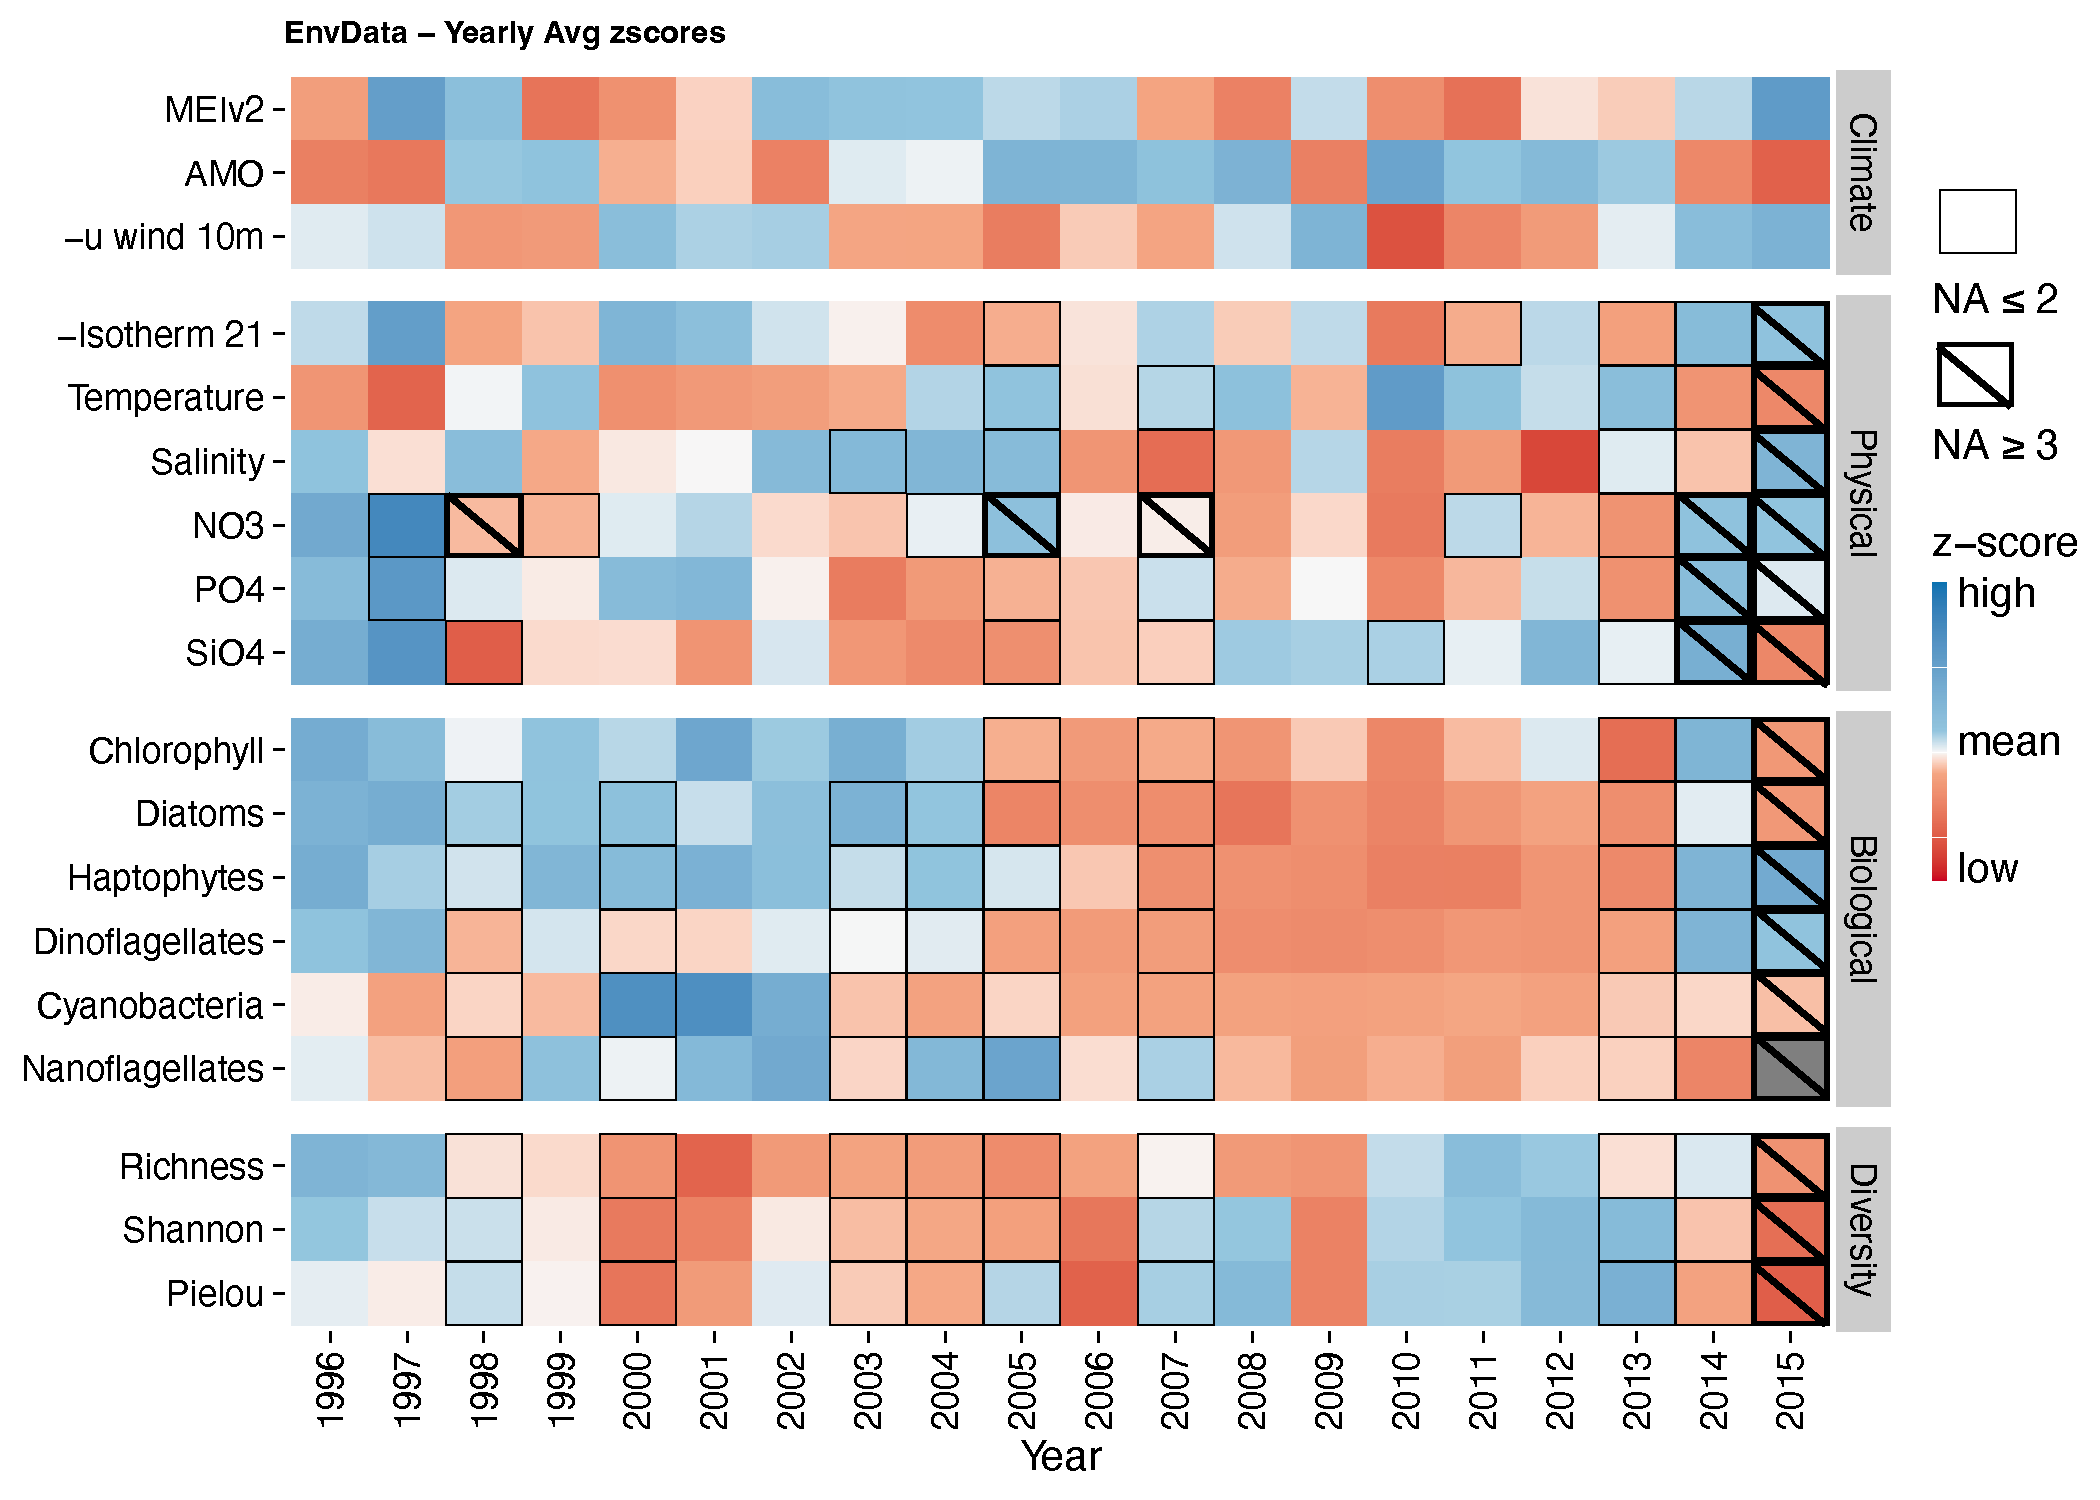
\includegraphics[width=\textwidth]{fig/PLOTZScores_updated.pdf}
\caption{Heatmap of yearly average values, normalized for comparison as z-scores. All data is available at monthly resolution (see next draft figure for raw data). Red indicates a larger value, blue indicates a smaller value for that particular year. The years 1995 (n=2) and 2017 (n=1) were removed due to lack of data. Diversity Indices are calculated based on microscopy counts at the Genus level.}
\end{figure}

\begin{figure}
\label{fig:divts}
\begin{center}
\noindent\includegraphics[width=480]{fig/DepthDivTimeSeries_updated.pdf}
\end{center}
\caption{Overview over Chlorophyll and Diversity Variables over Depth}
\end{figure}



\begin{figure}
\label{fig:clustering}
\noindent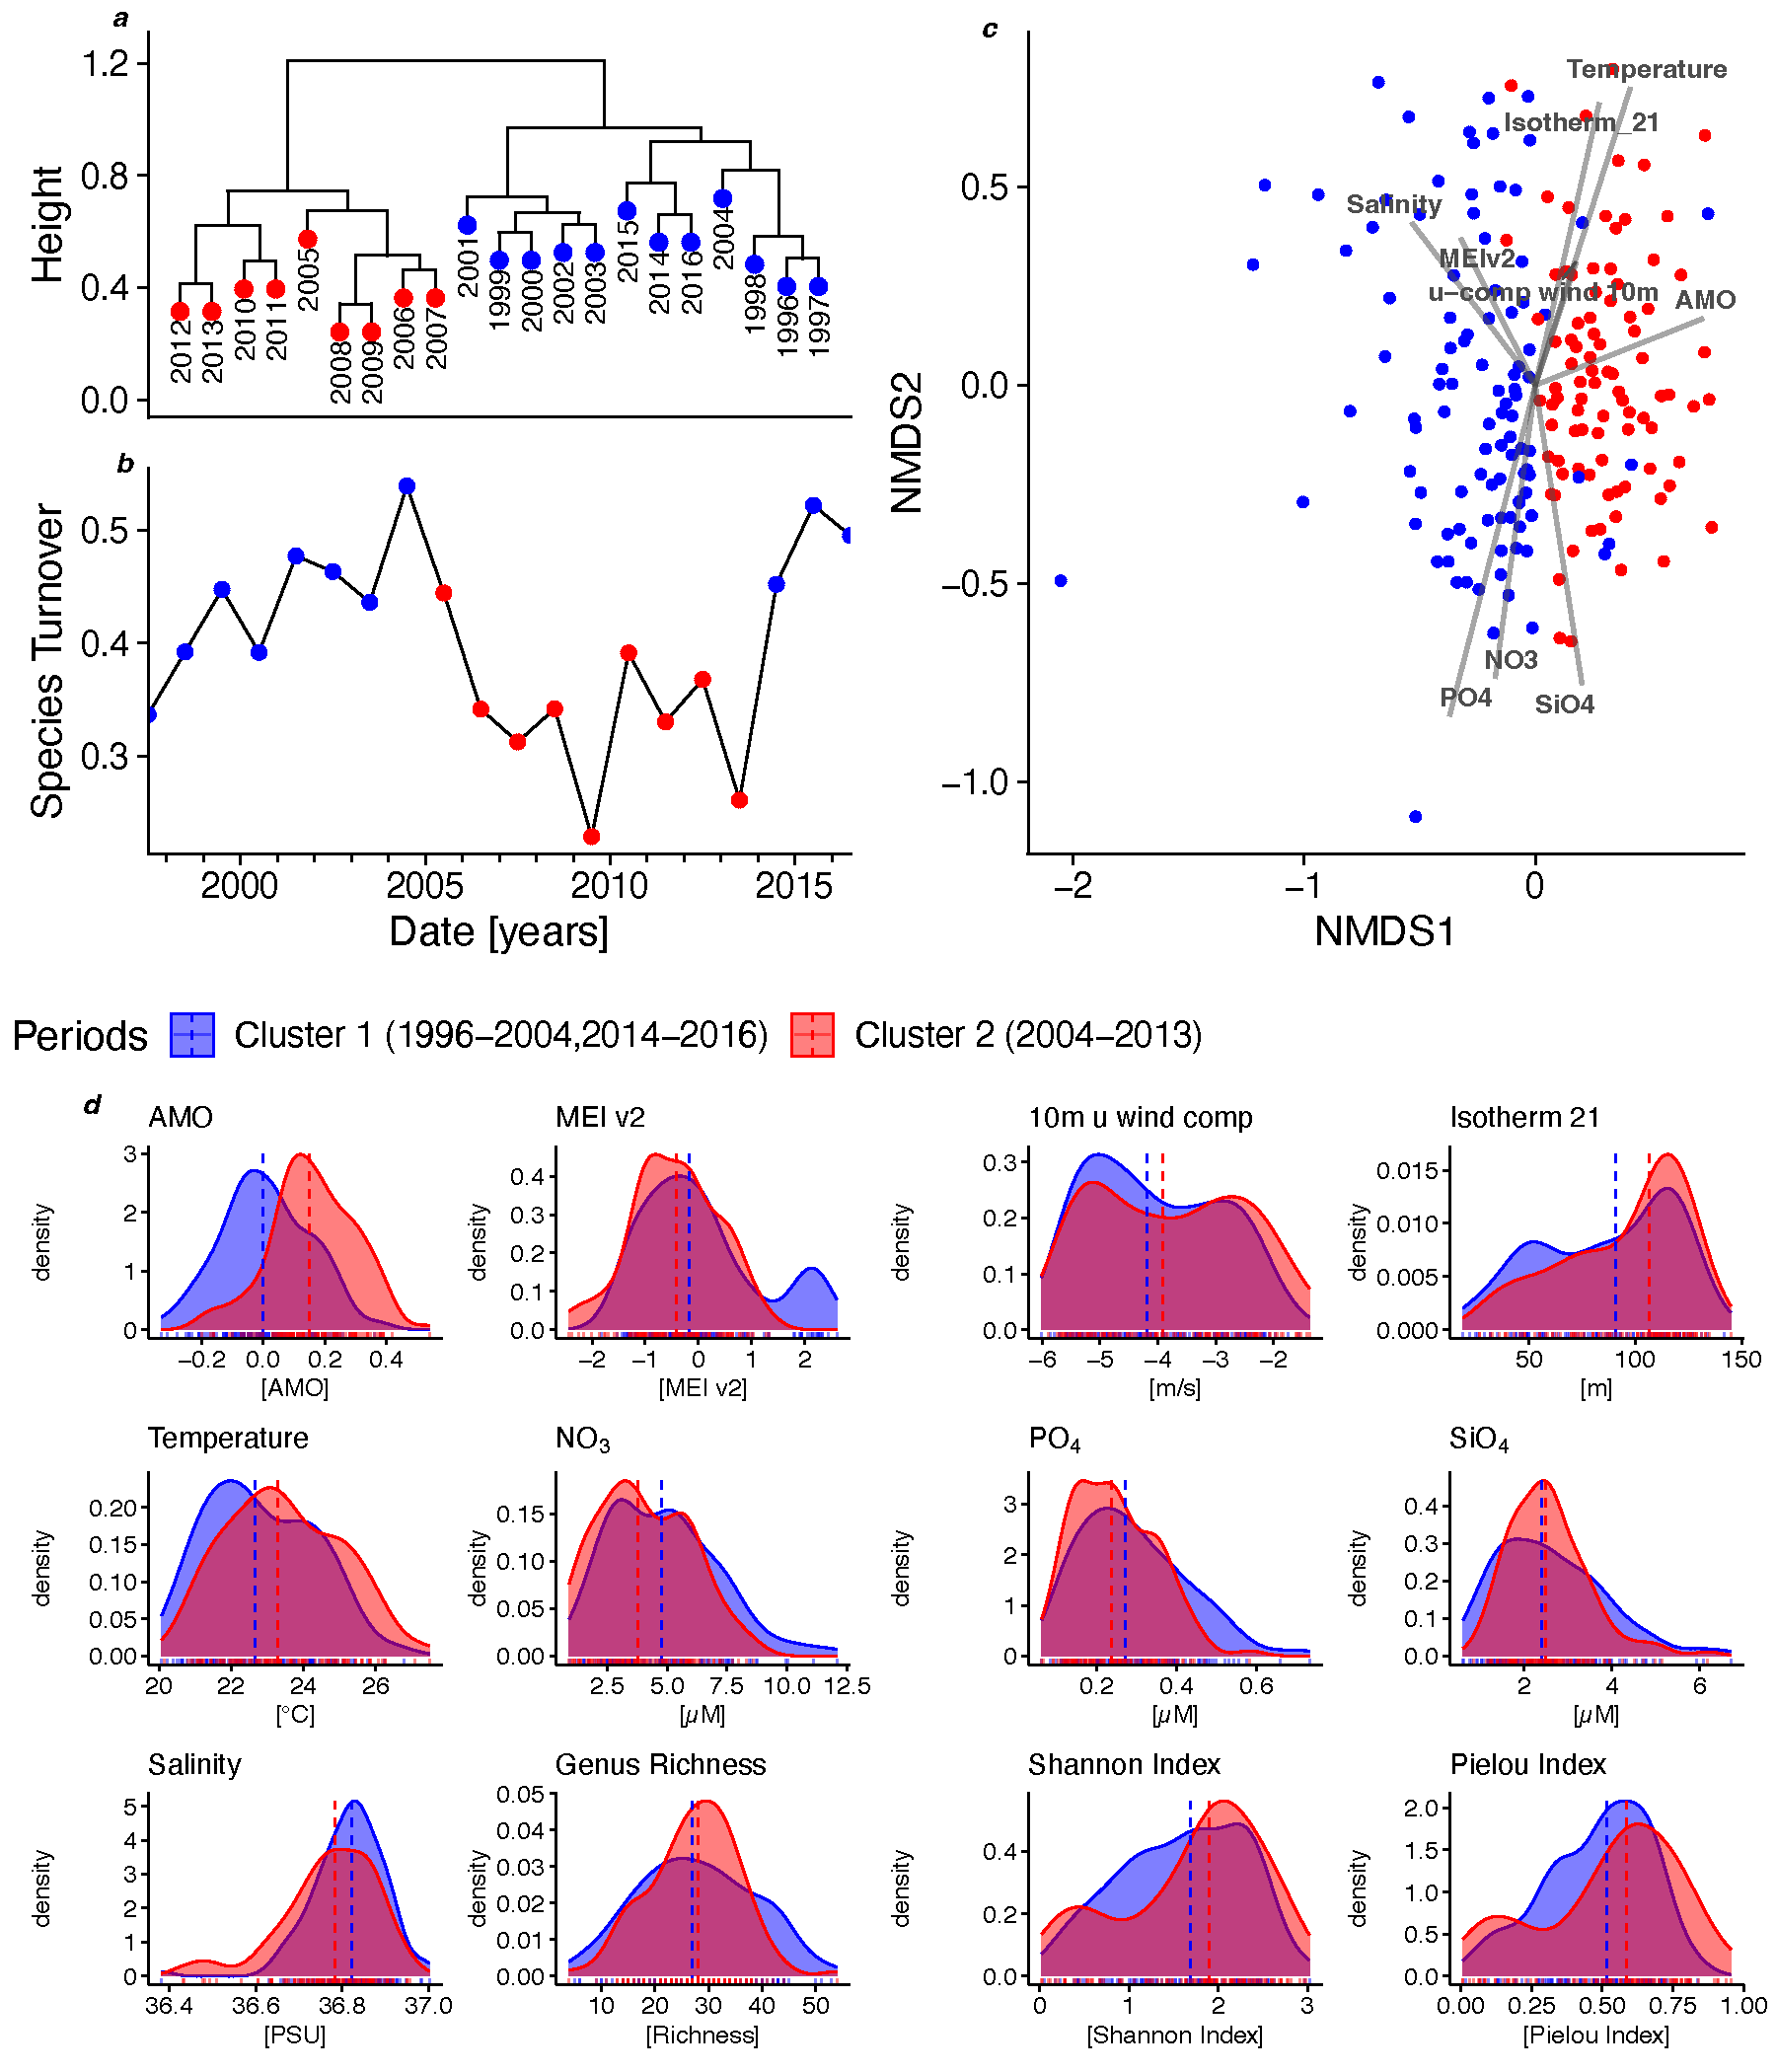
\includegraphics[width=\textwidth]{fig/ClusteringCompPlot_NEW.pdf}
\caption{(A) Clustering of microscopy data at the Genus level, using the binary Jaccard distance. The community for each year is binned together, to smooth out seasonal aspects. (B) NMDS plot of monthly community data (cell counts) that is cube root transformed. Stress: 0.261, 2 dimensions, converging solution. Color of dots based on which yearly cluster the monthly data is in. Vector overlay of ENVFIT shows underlying environmental variables that are co-varying with the community data.
Plots (A-L) below show density distributions of the environmental variables as well as diversity indices between the clustered years. Dashed line shows the mean.}
\end{figure}

\begin{table}
\label{table:clustering}
\caption{Wilcoxon sum rank test with continuity correction for variables between the two clusters. Values for in-situ data are interpolated across the top 100 meters for each individual monthly cruise sampling.}
\centering
\begin{tabular}[t]{lrrl}
\toprule
Variable & W & p.value & Significance\\
\midrule
AMO & 3494.0 & 1.86e-14 & ***\\
MEI v.2 & 9523.5 & 0.006 & ***\\
u-component 10 m wind speed & 7074.0 & 0.143 & n.s.\\
Isotherm 21 \degree C & 5293.0 & 0.034 & **\\
\addlinespace
Temperature & 4763.0 & 0.003 & ***\\
$NO_3$ & 6378.0 & 0.018 & **\\
$PO_4$ & 7359.0 & 0.012 & **\\
$SiO_4$ & 5998.0 & 0.736 & n.s.\\
Salinity & 7636.0 & 0.002 & ***\\
\addlinespace
Genus Richness & 5913.0 & 0.954 & n.s.\\
Shannon Index & 5142.0 & 0.108 & n.s.\\
Pielou Index & 4874.0 & 0.029 & **\\
\bottomrule
\end{tabular}
\end{table}


\begin{figure}
\label{fig:GF}
\noindent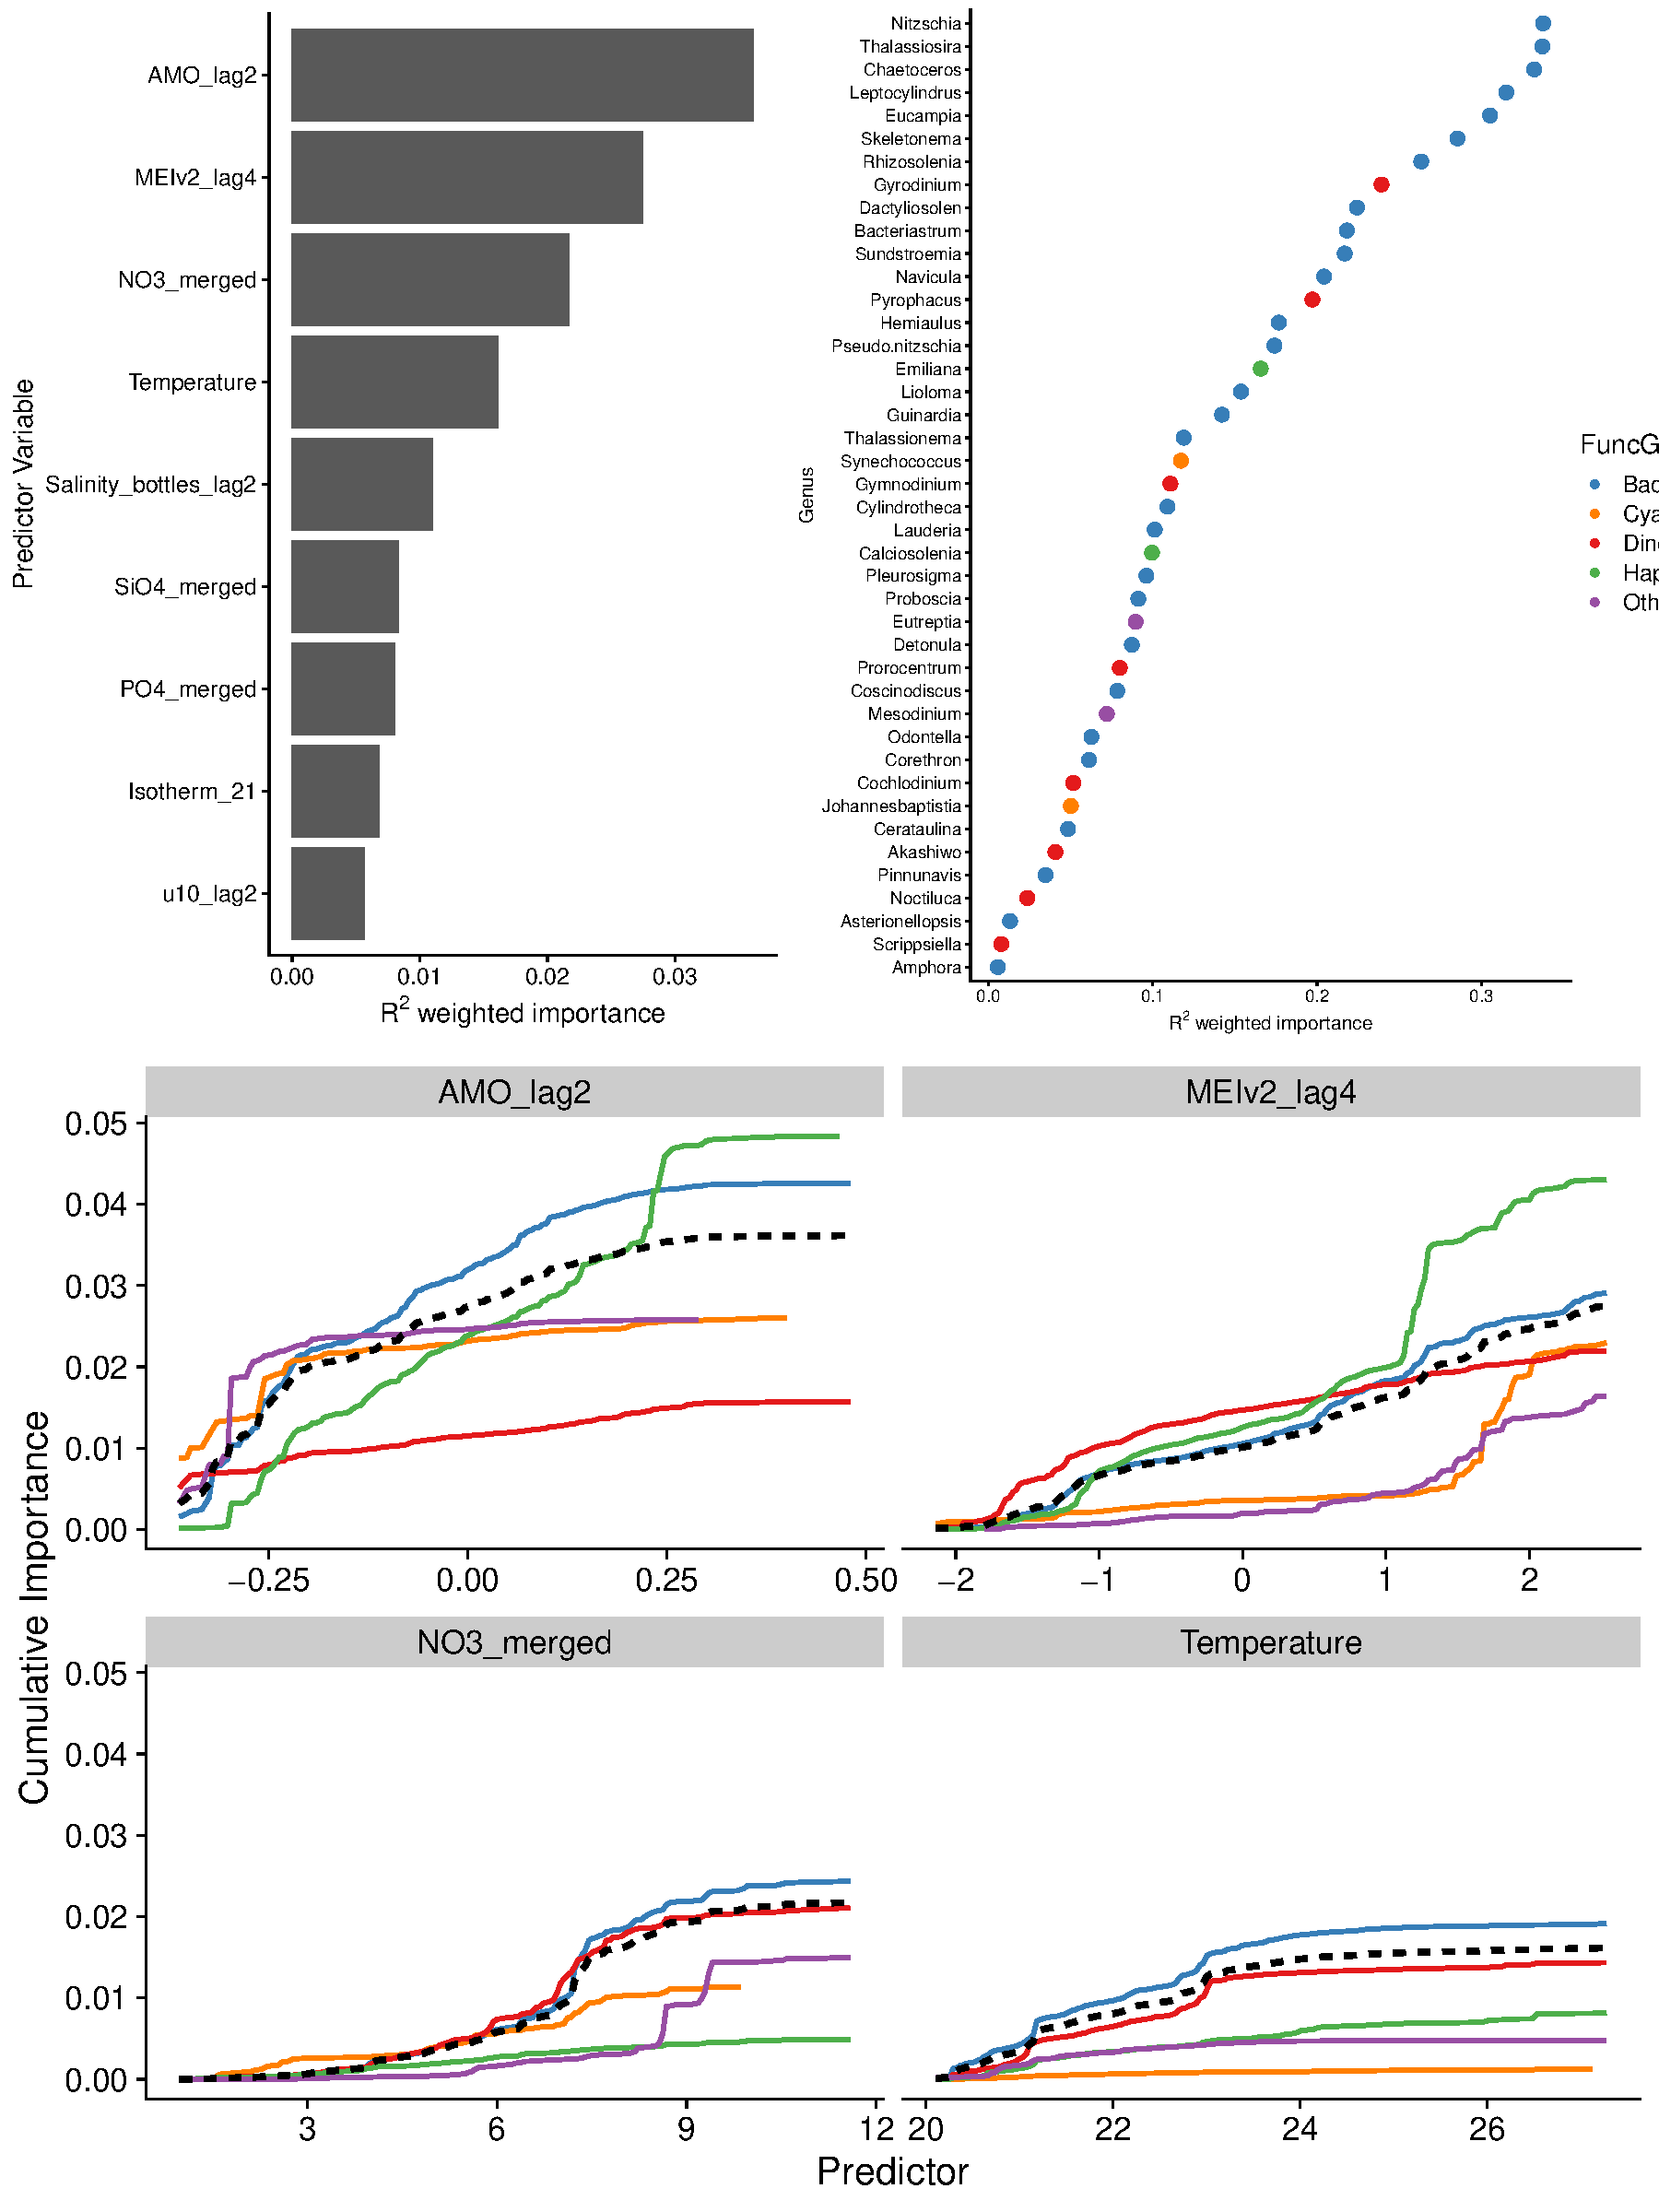
\includegraphics[width=\textwidth]{fig/GF_output_plot3_new.pdf}
\caption{Interestingly only time lags of the climatic indices (AMO and MEIv2) actually showed better predictive capabilities, there were none for lags of wind, nutrients or the isotherm. What I also included in the plot above is the underlying mechanism of fitting a random forest model for each genus. The plot on the top right shows the weighted importance for each genus, ranked according to the predictive capability of the model, and color coded by their respective group. Similarly, the cumulative importance plots below show the overall importance, as well as the individual color lines that show the cumulative importance per genus predicted. This is not necessarily useful to show in the final manuscript, unless we want to discuss the model output down to the genus level. Not surprisingly, it is mostly diatoms that are predictable, but also other groups are present here.}
\end{figure}


\section{Discussion}
This present study demonstrates the highly dynamic nature of a tropical coastal marine ecosystem, that is driven by local environmental variability, which is in turn affected by large scale climatic shifts. In the Cariaco basin, long-term climatic oscillations have affected the upwelling regime and ...
In the Cariaco basin, wind-driven seasonal upwelling dictates the nutrient availability in the upper mixed layer, which in turn affects the phytoplankton dynamics \cite{ptacnik_diversity_2008, bopp_response_2005}. In particular, Diatoms are responsive to changes in the mixing regime \cite{huisman_reduced_2006}.
Alterations in physical mixing affected phytoplankton dynamics,
% MEI index relevant (from 2019 REVIEW)
The Caribbean experiences the most marked of the El Niño–Southern Oscillation teleconnections in the Atlantic Ocean, with warmer sea surface temperatures and trade winds blowing more to the north-northwest during the El Niño–Southern Oscillation \cite{enfield_tropical_1997}.

% REALLY ONLY LOOK AT BOTTOM UP HERE; No Top Down effects quantified

\section{Conclusions}


%%

%  Numbered lines in equations:
%  To add line numbers to lines in equations,
%  \begin{linenomath*}
%  \begin{equation}
%  \end{equation}
%  \end{linenomath*}



%% Enter Figures and Tables near as possible to where they are first mentioned:
%
% DO NOT USE \psfrag or \subfigure commands.
%
% Figure captions go below the figure.
% Acronyms used in figure captions will be spelled out in the final, published version.

% Table titles go above tables;  other caption information
%  should be placed in last line of the table, using
% \multicolumn2l{$^a$ This is a table note.}
% NOTE that there is no difference between table caption and table heading in the final, published version
%
%----------------
% EXAMPLE FIGURES
%
% \begin{figure}
% \includegraphics{example.png}
% \caption{caption}
% \end{figure}
%
% Giving latex a width will help it to scale the figure properly. A simple trick is to use \textwidth. Try this if large figures run off the side of the page.
% \begin{figure}
% \noindent\includegraphics[width=\textwidth]{anothersample.png}
%\caption{caption}
%\label{pngfiguresample}
%\end{figure}
%
%
% If you get an error about an unknown bounding box, try specifying the width and height of the figure with the natwidth and natheight options. This is common when trying to add a PDF figure without pdflatex.
% \begin{figure}
% \noindent\includegraphics[natwidth=800px,natheight=600px]{samplefigure.pdf}
%\caption{caption}
%\label{pdffiguresample}
%\end{figure}
%
%
% PDFLatex does not seem to be able to process EPS figures. You may want to try the epstopdf package.
%

%
% ---------------
% EXAMPLE TABLE
%
% \begin{table}
% \caption{Time of the Transition Between Phase 1 and Phase 2$^{a}$}
% \centering
% \begin{tabular}{l c}
% \hline
%  Run  & Time (min)  \\
% \hline
%   $l1$  & 260   \\
%   $l2$  & 300   \\
%   $l3$  & 340   \\
%   $h1$  & 270   \\
%   $h2$  & 250   \\
%   $h3$  & 380   \\
%   $r1$  & 370   \\
%   $r2$  & 390   \\
% \hline
% \multicolumn{2}{l}{$^{a}$Footnote text here.}
% \end{tabular}
% \end{table}

%%%%%%%%%%%%%%%%%%%%%%%%%%%%%%%%%%%%%%%%%%%%%%%
% SIDEWAYS FIGURES and TABLES
% AGU prefers the use of {sidewaystable} over {landscapetable} as it causes fewer problems.
%
% \begin{sidewaysfigure}
% \includegraphics[width=20pc]{figsamp}
% \caption{caption here}
% \label{newfig}
% \end{sidewaysfigure}
%
%  \begin{sidewaystable}
%  \caption{Caption here}
% \label{tab:signif_gap_clos}
%  \begin{tabular}{ccc}
% one&two&three\\
% four&five&six
%  \end{tabular}
%  \end{sidewaystable}

%% If using numbered lines, please surround equations with \begin{linenomath*}...\end{linenomath*}
%\begin{linenomath*}
%\begin{equation}
%y|{f} \sim g(m, \sigma),
%\end{equation}
%\end{linenomath*}

%%% End of body of article

%%%%%%%%%%%%%%%%%%%%%%%%%%%%%%%%%%%%%%%%%%%%%%%
%% Optional Appendices go here
%
% The \appendix command resets counters and redefines section heads
%
% After typing \appendix
%
%\section{Here Is Appendix Title}
% will show
% A: Here Is Appendix Title
%

\appendix

\section{Gradient Forest Analysis supplement}


\begin{table}
\ref{app:table1}

\caption{Individual Gradient Forest model runs for each variable and the corresponding time lags. 
        For in-situ variables, for which no coverage extends over the time series, 
        we tested all measurements up to a lag of 3 months. 
        For climate variables, we tested up to a lag of 6 months. 
        Time lag with maximum importance per variable are highlighted in bold and chosen for the final model run.}
\centering
\begin{tabular}[t]{rrrrrrrrrr}
\toprule
lag & NO3 & PO4 & SiO4 & Temperature & Isotherm\_21 & Salinity\_bottles & u10 & AMO & MEIv2\\
\midrule
0 & \textbf{0.038} & \textbf{0.038} & \textbf{0.034} & \textbf{0.071} & \textbf{0.028} & 0.007 & 0.004 & 0.016 & 0.015\\
1 & 0.017 & 0.011 & 0.015 & 0.002 & 0.002 & 0.004 & \textbf{0.010} & 0.014 & 0.018\\
2 & 0.022 & 0.008 & 0.013 & 0.006 & 0.008 & \textbf{0.011} & 0.009 & \textbf{0.030} & 0.019\\
3 & 0.016 & 0.007 & 0.004 & 0.005 & 0.007 & 0.010 & 0.007 & 0.018 & 0.018\\
4 & - & - & - & - & - & - & 0.008 & 0.019 & \textbf{0.029}\\
5 & - & - & - & - & - & - & 0.008 & 0.018 & 0.022\\
6 & - & - & - & - & - & - & 0.010 & 0.018 & 0.013\\
\bottomrule
\end{tabular}
\end{table}


%%%%%%%%%%%%%%%%%%%%%%%%%%%%%%%%%%%%%%%%%%%%%%%
% Optional Glossary, Notation or Acronym section goes here:
%
% Glossary is only allowed in Reviews of Geophysics
%  \begin{glossary}
%  \term{Term}
%   Term Definition here
%  \term{Term}
%   Term Definition here
%  \term{Term}
%   Term Definition here
%  \end{glossary}


%%%%%%%%%%%%%%%%%%%%%%%%%%%%%%%%%%%%%%%%%%%%%%%
% Acronyms
%% NOTE that acronyms in the final published version will be spelled out when used in figure captions.
%   \begin{acronyms}
%   \acro{Acronym}
%   Definition here
%   \acro{EMOS}
%   Ensemble model output statistics
%   \acro{ECMWF}
%   Centre for Medium-Range Weather Forecasts
%   \end{acronyms}


%%%%%%%%%%%%%%%%%%%%%%%%%%%%%%%%%%%%%%%%%%%%%%%
% Notation
%   \begin{notation}
%   \notation{$a+b$} Notation Definition here
%   \notation{$e=mc^2$}
%   Equation in German-born physicist Albert Einstein's theory of special
%  relativity that showed that the increased relativistic mass ($m$) of a
%  body comes from the energy of motion of the body—that is, its kinetic
%  energy ($E$)—divided by the speed of light squared ($c^2$).
%   \end{notation}




%%%%%%%%%%%%%%%%%%%%%%%%%%%%%%%%%%%%%%%%%%%%%%%
%
% DATA SECTION and ACKNOWLEDGMENTS
%
%%%%%%%%%%%%%%%%%%%%%%%%%%%%%%%%%%%%%%%%%%%%%%%

%!
\section*{Open Research Section}
This section MUST contain a statement that describes where the data supporting the conclusions can be obtained. Data cannot be listed as ''Available from authors'' or stored solely in supporting information. Citations to archived data should be included in your reference list. Wiley will publish it as a separate section on the paper’s page. Examples and complete information are here:
https://www.agu.org/Publish with AGU/Publish/Author Resources/Data for Authors

\section*{As Applicable – Inclusion in Global Research Statement}
The Authorship: Inclusion in Global Research policy aims to promote greater equity and transparency in research collaborations. AGU Publications encourage research collaborations between regions, countries, and communities and expect authors to include their local collaborators as co-authors when they meet the AGU Publications authorship criteria (described here: https://www.agu.org/publications/authors/policies\#authorship). Those who do not meet the criteria should be included in the Acknowledgement section. We encourage researchers to consider recommendations from The TRUST CODE - A Global Code of Conduct for Equitable Research Partnerships (https://www.globalcodeofconduct.org/) when conducting and reporting their research, as applicable, and encourage authors to include a disclosure statement pertaining to the ethical and scientific considerations of their research collaborations in an “Inclusion in Global Research Statement’ as a standalone section in the manuscript following the Conclusions section. This can include disclosure of permits, authorizations, permissions and/or any formal agreements with local communities or other authorities, additional acknowledgements of local help received, and/or description of end-users of the research. You can learn more about the policy in this editorial. Example statements can be found in the following published papers: 
%Holt et al. (https://agupubs.onlinelibrary.wiley.com/doi/full/10.1029/2022JG007188), 
%Sánchez-Gutiérrez et al. (https://agupubs.onlinelibrary.wiley.com/doi/abs/10.1029/2023JG007554), 
%Tully et al. (https://agupubs.onlinelibrary.wiley.com/doi/epdf/10.1029/2022JG007128) 
%Please note that these statements are titled as “Global Research Collaboration Statements” from a previous pilot requirement in JGR Biogeosciences. The pilot has ended and statements should now be titled “Inclusion in Global Research Statement”.


%!
\acknowledgments
Thank you to all who have helped, communicated, provided data. Claudia Benitez-Nelson, Digna Rueda-Roa, James Pinckney.

%Enter acknowledgments here. This section is to acknowledge funding, thank colleagues, enter any secondary affiliations, and so on.


%%%%%%%%%%%%%%%%%%%%%%%%%%%%%%%%%%%%%%%%%%%%%%%
% REFERENCES and BIBLIOGRAPHY
%
%\bibliography{<name of your .bib file>} don't specify the file extension
% don't specify bibliographystyle
%
%%%%%%%%%%%%%%%%%%%%%%%%%%%%%%%%%%%%%%%%%%%%%%%

\bibliography{references}



%Reference citation instructions and examples:
%
% Please use ONLY \cite and \citeA for reference citations.
% \cite for parenthetical references
% ...as shown in recent studies (Simpson et al., 2019)
% \citeA for in-text citations
% ...Simpson et al. (2019) have shown...
%
%
%...as shown by \citeA{jskilby}.
%...as shown by \citeA{lewin76}, \citeA{carson86}, \citeA{bartoldy02}, and \citeA{rinaldi03}.
%...has been shown \cite{jskilbye}.
%...has been shown \cite{lewin76,carson86,bartoldy02,rinaldi03}.
%... \cite <i.e.>[]{lewin76,carson86,bartoldy02,rinaldi03}.
%...has been shown by \cite <e.g.,>[and others]{lewin76}.
%
% apacite uses < > for prenotes and [ ] for postnotes
% DO NOT use other cite commands (e.g., \citet, \citep, \citeyear, \nocite, \citealp, etc.).
%




\end{document}



More Information and Advice:

%%%%%%%%%%%%%%%%%%%%%%%%%%%%%%%%%%%%%%%%%%%%%%%
%
%  SECTION HEADS
%
%%%%%%%%%%%%%%%%%%%%%%%%%%%%%%%%%%%%%%%%%%%%%%%

% Capitalize the first letter of each word (except for
% prepositions, conjunctions, and articles that are
% three or fewer letters).

% AGU follows standard outline style; therefore, there cannot be a section 1 without
% a section 2, or a section 2.3.1 without a section 2.3.2.
% Please make sure your section numbers are balanced.
% ---------------
% Level 1 head
%
% Use the \section{} command to identify level 1 heads;
% type the appropriate head wording between the curly
% brackets, as shown below.
%
%An example:
%\section{Level 1 Head: Introduction}
%
% ---------------
% Level 2 head
%
% Use the \subsection{} command to identify level 2 heads.
%An example:
%\subsection{Level 2 Head}
%
% ---------------
% Level 3 head
%
% Use the \subsubsection{} command to identify level 3 heads
%An example:
%\subsubsection{Level 3 Head}
%
%---------------
% Level 4 head
%
% Use the \subsubsubsection{} command to identify level 3 heads
% An example:
%\subsubsubsection{Level 4 Head} An example.
%
%%%%%%%%%%%%%%%%%%%%%%%%%%%%%%%%%%%%%%%%%%%%%%%
%
%  IN-TEXT LISTS
%
%%%%%%%%%%%%%%%%%%%%%%%%%%%%%%%%%%%%%%%%%%%%%%%
%
% Do not use bulleted lists; enumerated lists are okay.
% \begin{enumerate}
% \item
% \item
% \item
% \end{enumerate}
%
%%%%%%%%%%%%%%%%%%%%%%%%%%%%%%%%%%%%%%%%%%%%%%%
%
%  EQUATIONS
%
%%%%%%%%%%%%%%%%%%%%%%%%%%%%%%%%%%%%%%%%%%%%%%%

% Single-line equations are centered.
% Equation arrays will appear left-aligned.

Math coded inside display math mode \[ ...\]
 will not be numbered, e.g.,:
 \[ x^2=y^2 + z^2\]

 Math coded inside \begin{equation} and \end{equation} will
 be automatically numbered, e.g.,:
 \begin{equation}
 x^2=y^2 + z^2
 \end{equation}


% To create multiline equations, use the
% \begin{eqnarray} and \end{eqnarray} environment
% as demonstrated below.
\begin{eqnarray}
  x_{1} & = & (x - x_{0}) \cos \Theta \nonumber \\
        && + (y - y_{0}) \sin \Theta  \nonumber \\
  y_{1} & = & -(x - x_{0}) \sin \Theta \nonumber \\
        && + (y - y_{0}) \cos \Theta.
\end{eqnarray}

%If you don't want an equation number, use the star form:
%\begin{eqnarray*}...\end{eqnarray*}

% Break each line at a sign of operation
% (+, -, etc.) if possible, with the sign of operation
% on the new line.

% Indent second and subsequent lines to align with
% the first character following the equal sign on the
% first line.

% Use an \hspace{} command to insert horizontal space
% into your equation if necessary. Place an appropriate
% unit of measure between the curly braces, e.g.
% \hspace{1in}; you may have to experiment to achieve
% the correct amount of space.


%%%%%%%%%%%%%%%%%%%%%%%%%%%%%%%%%%%%%%%%%%%%%%%
%
%  EQUATION NUMBERING: COUNTER
%
%%%%%%%%%%%%%%%%%%%%%%%%%%%%%%%%%%%%%%%%%%%%%%%

% You may change equation numbering by resetting
% the equation counter or by explicitly numbering
% an equation.

% To explicitly number an equation, type \eqnum{}
% (with the desired number between the brackets)
% after the \begin{equation} or \begin{eqnarray}
% command.  The \eqnum{} command will affect only
% the equation it appears with; LaTeX will number
% any equations appearing later in the manuscript
% according to the equation counter.
%

% If you have a multiline equation that needs only
% one equation number, use a \nonumber command in
% front of the double backslashes (\\) as shown in
% the multiline equation above.

% If you are using line numbers, remember to surround
% equations with \begin{linenomath*}...\end{linenomath*}

%  To add line numbers to lines in equations:
%  \begin{linenomath*}
%  \begin{equation}
%  \end{equation}
%  \end{linenomath*}



